\documentclass[12pt]{article}
\usepackage[utf8]{inputenc}
\usepackage{float}
\usepackage{amsmath}
\usepackage{tikz}


\usepackage[hmargin=3cm,vmargin=6.0cm]{geometry}
%\topmargin=0cm
\topmargin=-2cm
\addtolength{\textheight}{6.5cm}
\addtolength{\textwidth}{2.0cm}
%\setlength{\leftmargin}{-5cm}
\setlength{\oddsidemargin}{0.0cm}
\setlength{\evensidemargin}{0.0cm}

%misc libraries goes here



\begin{document}

\section*{Student Information } 
%Write your full name and id number between the colon and newline
%Put one empty space character after colon and before newline
Full Name : Aybüke Aksoy \\
Id Number : 2448090 \\

% Write your answers below the section tags
\section*{Answer 1}
$a_n=a_{n-1}+2^n , \ n \geq 1, \ a_0=1$\\
$(a_0,a_1,a_2,......a_n)=(1,3,7....)$\\\\
To find the general rule for
$a_n$\\
$\sum_{n=1}^{\infty} a_n \cdot x^n=\sum_{n=1}^{\infty} (a_{n-1} + 2^n) \cdot x^n$\\\\
where 
$A(x)=\sum_{n=0}^{\infty} a_n \cdot x^n;$\\
$\sum_{n=1}^{\infty} a_n \cdot x^n=A(x)-a_0$\\
$A(x)-a_0=\sum_{n=1}^{\infty} a_{n-1} \cdot x^n + \sum_{n=1}^{\infty} 2^n \cdot x^n$\\
$A(x)-a_0=x \cdot \sum_{n=1}^{\infty} a_{n-1} \cdot x^{n-1} + \sum_{n=1}^{\infty} 2^n \cdot x^n$\\\\
Since 
$\sum_{n=1}^{\infty} a_{n-1} \cdot x^{n-1}=\sum_{n=0}^{\infty} a_n=A(x);$\\
$A(x)-a_0=x \cdot A(x)+ \sum_{n=1}^{\infty} 2^n \cdot x^n$\\
$A(x)-a_0=x \cdot A(x)+ \sum_{n=1}^{\infty} (2x)^n$\\
$\sum_{n=1}^{\infty} (2x)^n=\sum_{n=0}^{\infty} (2x)^n-1 \ as \ (2x)^n \ where \ n=0 \ is \ 1.$\\
$\sum_{n=0}^{\infty} (2x)^n=1/(1-2x)$\\\\
$A(x)-1=x \cdot A(x) + 1/(1-2x) -1$\\
$A(x)=x \cdot A(x) + 1/(1-2x)$\\
$A(x)-x \cdot A(x) = 1/(1-2x)$\\
$A(x) \cdot (1-x)=1/(1-2x)$\\
$A(x)=1/((1-2x) \cdot (1-x))$\\\\
$A(x)=A/(1-2x)+B/(1-x)=1/((1-2x) \cdot (1-x))$
where A and B are constants.\\
$A \cdot (1-x) + B \cdot (1-2x)=1$\\
$A-A \cdot x + B-2B \cdot x=1$\\
$x \cdot (-A-2B)+A+B=1$\\
$-A-2B=0 \ and \ A+B=1$\\
A=2 , B=-1\\\\
$A(x)=2/(1-2x)+ -1/(1-x)$\\
$-1/(1-x) \iff (-1,-1,-1,-1.....-1^n)$\\
$2/(1-2x) \iff (2,4,8,16......2^{n+1})$\\
$A(x)=2/(1-2x)+ -1/(1-x) \iff (1,3,7,15....2^{n+1}-1)$\\
$a_n=2^{n+1}-1$\\

\section*{Answer 2}
Given the relation R =
$\{(a, b)\ |\ a \ divides \ b\} \ on \ A = \{1, 2, 3, 9, 18\};$\\\\
a) Hasse Diagram of R:\\\\
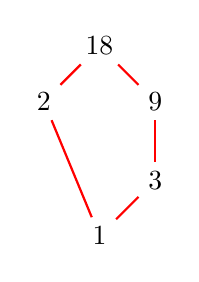
\begin{tikzpicture}
    \node (top) at (0,0) {$18$};
    \node [below left  of=top] (left)  {$2$};
\node [below right of=top] (right) {$9$};
\node [below of=right] (belowright) {$3$};
\node [below left of=belowright] (leftbelow) {$1$};
\draw [red,  thick] (top) -- (left);
\draw [red,  thick] (top) -- (right);
\draw [red,  thick] (right) -- (belowright);
\draw [red,  thick] (belowright) -- (leftbelow);
\draw [red,  thick] (left) -- (leftbelow);
\end{tikzpicture}\\\\
b) Matrix representation for R:\\\\
$M_R=$
\begin{bmatrix}
    1      & 1 & 1 & 1 & 1 \\
    0     & 1 & 0 & 0 & 1 \\
    0      & 0 & 1 & 1 & 1 \\
    0     & 0 & 0 & 1 & 1 \\
    0      & 0 & 0 & 0 & 1 \\
    
\end{bmatrix}\\\\\\
c)Yes it is a lattice. A lattice is a poset in which every pair of elements has both a least upper bound and a greatest lower bound. \\
(A,R) is a lattice since every pair of elements in our poset has both a least upper and greatest lower bound.\\
Pairs with their LUBs and GLBs:\\
(1,2) $\rigtharrow$  LUB: 2 ,  GLB: 1\\
(1,3) $\rigtharrow$   LUB: 3 ,  GLB: 1\\
(1,9) $\rigtharrow$   LUB: 9 ,  GLB: 1\\
(1,18) $\rigtharrow$   LUB: 18 ,  GLB: 1\\
(2,3) $\rigtharrow$   LUB: 18,  GLB: 1\\
(2,9) $\rigtharrow$   LUB: 18 ,  GLB: 1\\
(2,18) $\rigtharrow$   LUB: 18 ,  GLB: 2\\
(3,9) $\rigtharrow$   LUB: 9 ,  GLB: 3\\
(3,18) $\rigtharrow$   LUB: 18 ,  GLB: 3\\
(9,18) $\rigtharrow$   LUB: 18,  GLB: 9\\
.......\\\\\\
d) 
$R_s=$
$R \cup R^{-1}$
where 
$R^{-1}=\{(b,a) | (a,b)\in R\} $\\\\
$M_{R^{-1}}=M_R^T=$
\begin{bmatrix}
    1      & 0 & 0 & 0 & 0 \\
    1    & 1 & 0 & 0 & 0 \\
    1      & 0 & 1 & 0 & 0 \\
    1     & 0 & 1 & 1 & 0 \\
    1      & 1 & 1 & 1 & 1 \\
    
\end{bmatrix}\\\\\\
Matrix representation for 
$R_s=M_s=M_R \lor M_{R^{-1}}$\\\\
Ms=
\begin{bmatrix}
    1      & 1 & 1 & 1 & 1 \\
    0     & 1 & 0 & 0 & 1 \\
    0      & 0 & 1 & 1 & 1 \\
    0     & 0 & 0 & 1 & 1 \\
    0      & 0 & 0 & 0 & 1 \\
    
\end{bmatrix}
\lor
\begin{bmatrix}
    1      & 0 & 0 & 0 & 0 \\
    1    & 1 & 0 & 0 & 0 \\
    1      & 0 & 1 & 0 & 0 \\
    1     & 0 & 1 & 1 & 0 \\
    1      & 1 & 1 & 1 & 1 \\
    
\end{bmatrix}
=
\begin{bmatrix}
    1      & 1 & 1 & 1 & 1 \\
    1    & 1 & 0 & 0 & 1 \\
    1      & 0 & 1 & 1 & 1 \\
    1     & 0 & 1 & 1 & 1 \\
    1      & 1 & 1 & 1 & 1 \\
    
\end{bmatrix}\\\\\\

e)
For this binary relation, two integers a and b are comparable if
$a \ | \ b \ or \ b \ | \ a.$\\
Since 
$\ 2 \not | \ 9$
and
$9 \not | \ 2$
and neither divides the other, the integers 2 and 9 are uncomparable in (A,R). However; even if 
$18 \not | \ 3,$
since
$3 | 18, $ 
the integers 3 and 18 are comparable in (A,R).



\section*{Answer 3}

a) $2^n \cdot 3{n \cdot (n-1)/2}$\\\\
Let's think of a matrix representation of a binary relation on a set A with n elements.\\Any anti-symmetric relation has no restriction on the reflexivity. Therefore, the main diagonal elements of the matrix can be either 0 or 1. It means we have 2 options for each element on the main diagonal. By the product rule, we have
$2^n$
ways to construct the diagonal. 
Then, if we choose an element 
$a_{ij}$ 
from the upper right triangle, its symmetric element 
$a_{ji}$
on the left lower triangle must be related to  
$a_{ij}.$\\
We have 3 alternatives that satisfies the anti-symmetric properties:\\
$a_{ij}=0 , a_{ji}=1$\\
$a_{ij}=1 , a_{ji}=0$\\
$a_{ij}=0 , a_{ji}=0$\\
The number of elements we have on the upper right triangle is total number of elements - number of main diagonal elements divided by 2;\\
$(n^2-n)/2=n \cdot (n-1)/2$\\
This is equal to number of pairs we have like
$(a_{ij},a_{ji})$
and for each possible pair, we have 3 options. By the product rule, we have
$3^{n \cdot (n-1)/2}$
ways to construct the matrix except the diagonal.\\
Thus, in total we have
$2^n \cdot 3^{n \cdot (n-1)/2}$ 
ways for the whole matrix and this gives us the number of different binary relations on A that are anti-symmetric.\\
Matrix example for one of the anti-symmetric binary relations on A
\begin{bmatrix}
    1     & 1 & 0 & 0 & 0 \\
    0    & 1 & 0 & 0 & 0 \\
    1      & 0 & 0 & 0 & 0 \\
    1     & 0 & 1 & 1 & 1 \\
    1      & 1 & 1 & 0 & 1 \\
    
\end{bmatrix}\\\\
b) $3^{n \cdot (n-1)/2}$\\\\
As we did in part a, we can again think of the matrix representation.\\
This time, we have a restriction on reflexivity and reflexive relations are represented by a matrix that has 1 on the main diagonal since every element must have a relation to itself. Therefore, we have only 1 way to construct the diagonal.\\ 
For anti-symmetry, we have the same 3 alternatives from part a  for each pair like 
$(a_{ij},a_{ji})$
and this again gives us
$3^{n \cdot (n-1)/2}$
ways to construct the rest of the matrix. 
Hence, in total we have, 
$3^{n \cdot (n-1)/2}$
ways for the whole matrix and this gives us the number of different binary relations on A that are both reflexive and anti-symmetric.\\
Matrix example for one of the reflexive and anti-symmetric binary relations on A
\begin{bmatrix}
    1     & 1 & 0 & 0 & 0 \\
    0    & 1 & 0 & 0 & 0 \\
    1      & 0 & 1 & 0 & 0 \\
    1     & 0 & 1 & 1 & 1 \\
    1      & 1 & 1 & 0 & 1 \\
    
\end{bmatrix}\\\\






\end{document}